%This is an appendix
\section{Placement optimisation for \textit{Needed} return policy}
\label{sec:needed}

 
 \begin{figure}[h]
     \centering     %%% not \center
    \subfloat[][Percentage of infeasible trips. Y-Axis is logarithmic.]
    {
        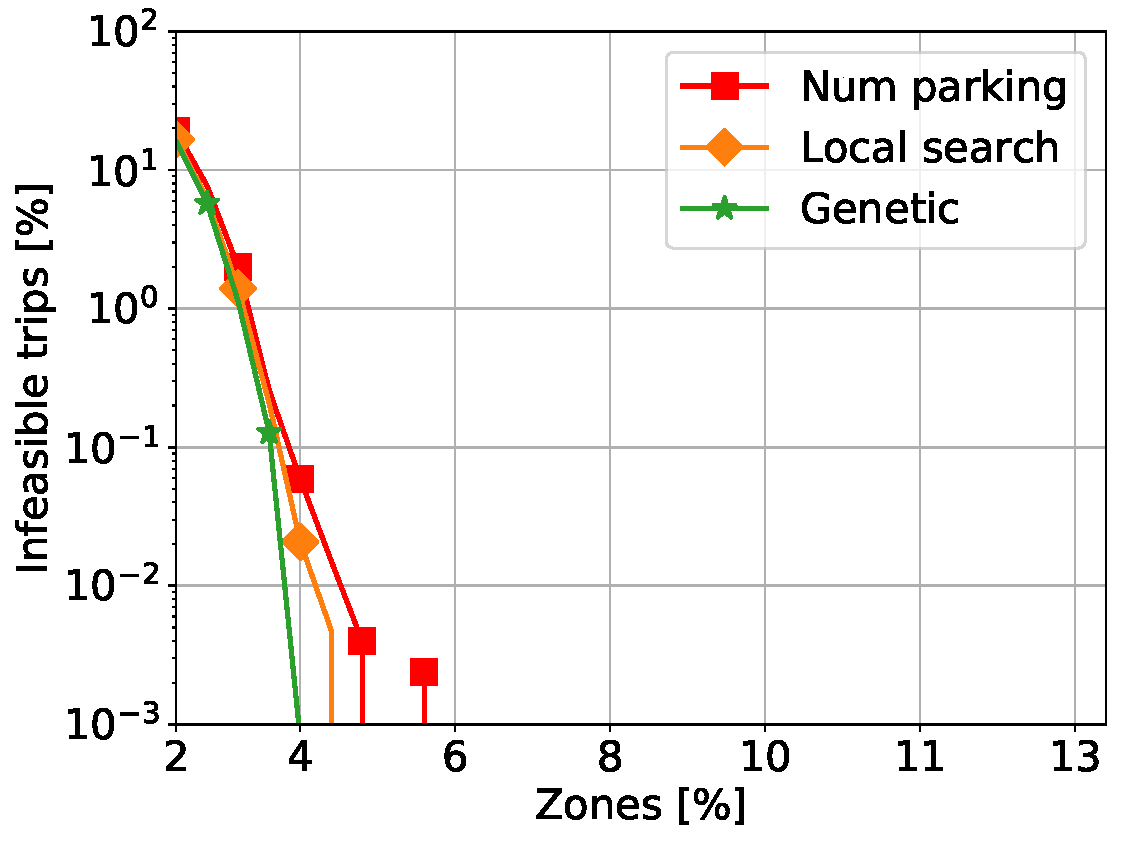
\includegraphics[width=0.45\textwidth]{figures/Needed_Deaths.pdf}
        \label{fig:optimized_deaths_Needed}
    }     
     \subfloat[][Walked distance, averaged over all trips.]
     {
         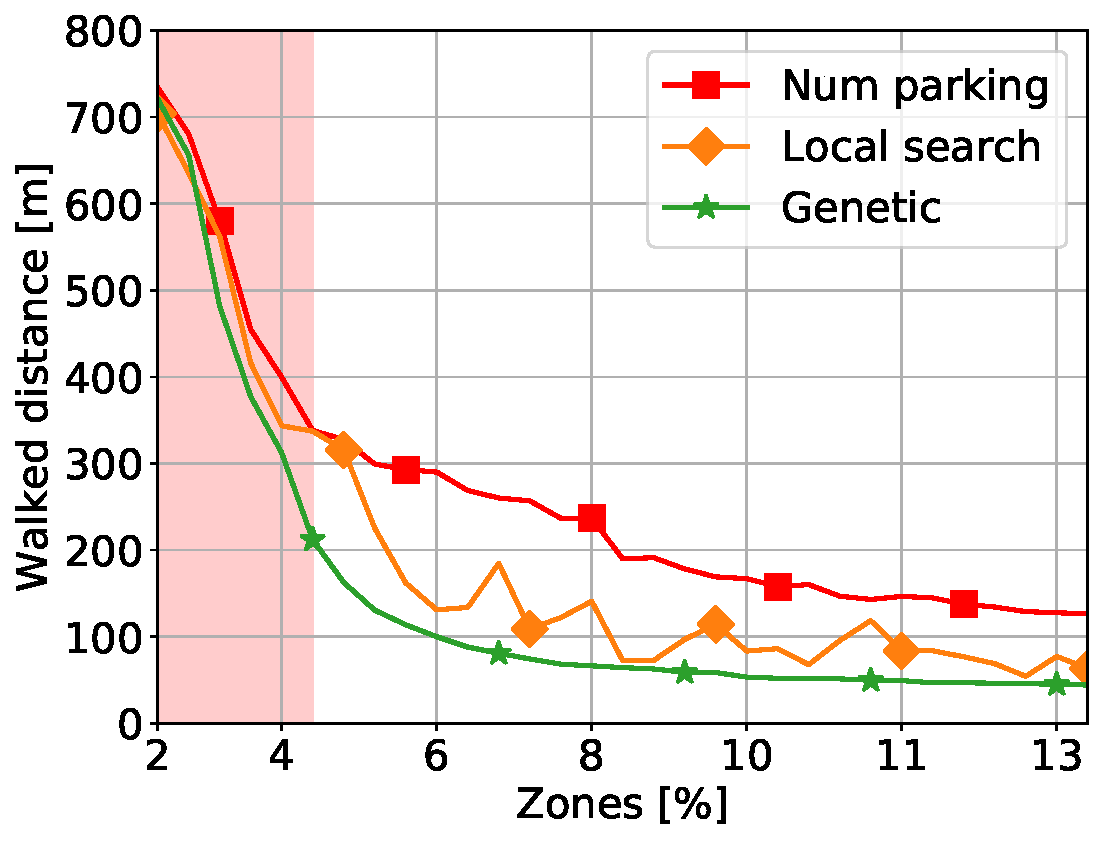
\includegraphics[width=0.45\textwidth]{figures/Needed_TravelWithPenlaty.pdf}
         \label{fig:wwd_Needed}
     }
     \caption{Objective metrics to minimise in the optimisation - with \textit{Needed} return policy}
    \label{fig:optimized_metrics_needed}
 \end{figure}
 
Here  we briefly report the results for the optimisation experiments of the \textit{Needed} policy.
We followed the same procedure explained in Sec.~\ref{sec:opt} for the \textit{Hybrid} return policy. As in that case, the genetic algorithm is able to largely optimise the solution, as reported in Fig.~\ref{fig:optimized_metrics_needed}, with \textit{local searches} stuck in local minima. 
In particular, for the walked distance (Fig.~\ref{fig:wwd_Needed}), the genetic algorithm is able lower it from 136\,m to 45\,m at 13\% of zones. Still, it doesn't reach the performance of the \textit{Hybrid} policy, i.e., 30\,m at 13\% of zones.


%Fig.~\ref{fig:optimized_deaths_Needed}, the infeasible trips perform better with the \textit{Genetic} and the \textit{Local search} getting to zero infeasible trips with \dg{4.3}\% and \dg{7.7}  respectively.
%Looking at the walked distance in Fig.~\ref{fig:wwd_Needed}, we can see that both optimizers perform much better with respect to the \textit{Num Parking} getting lower than 100 m. 

  \begin{figure}[t]
     \subfloat[][Charges percentage.]
     {
         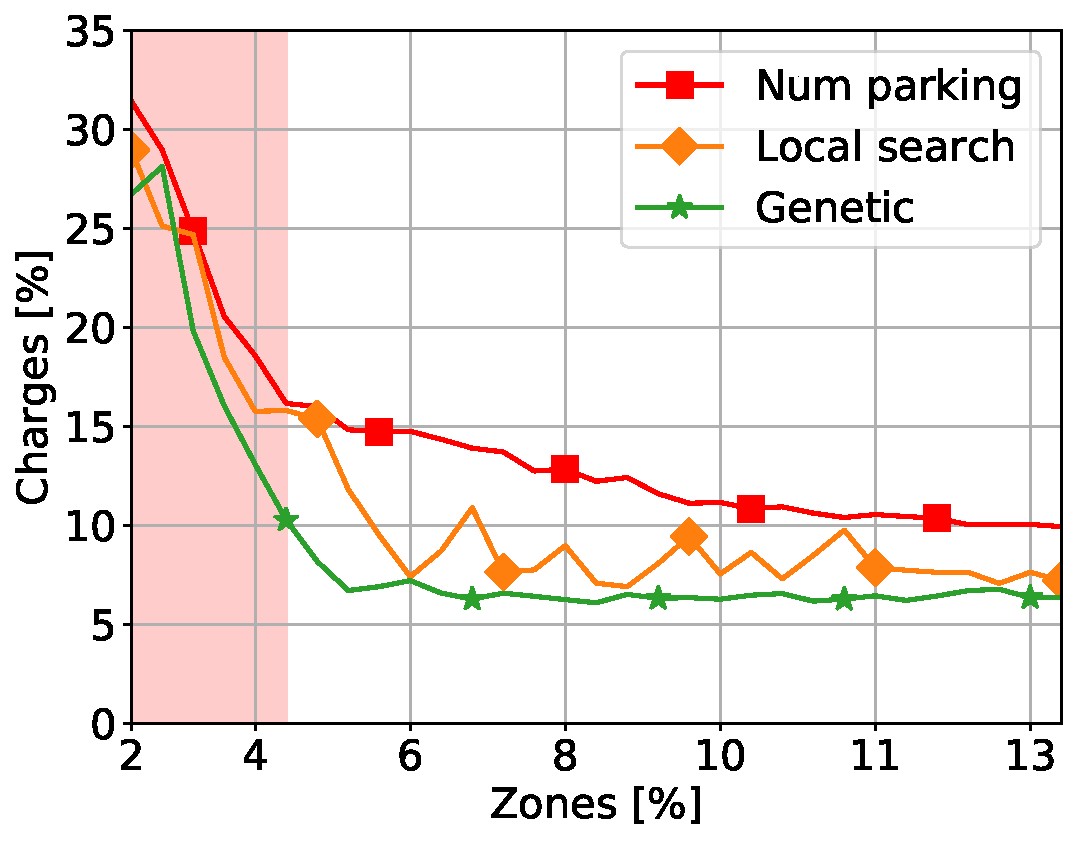
\includegraphics[width=0.45\textwidth]{figures/Needed_AmountRechargePerc.pdf}
         \label{fig:recharge_Needed}
     }
    \subfloat[][Average state of charge.]
    {         
        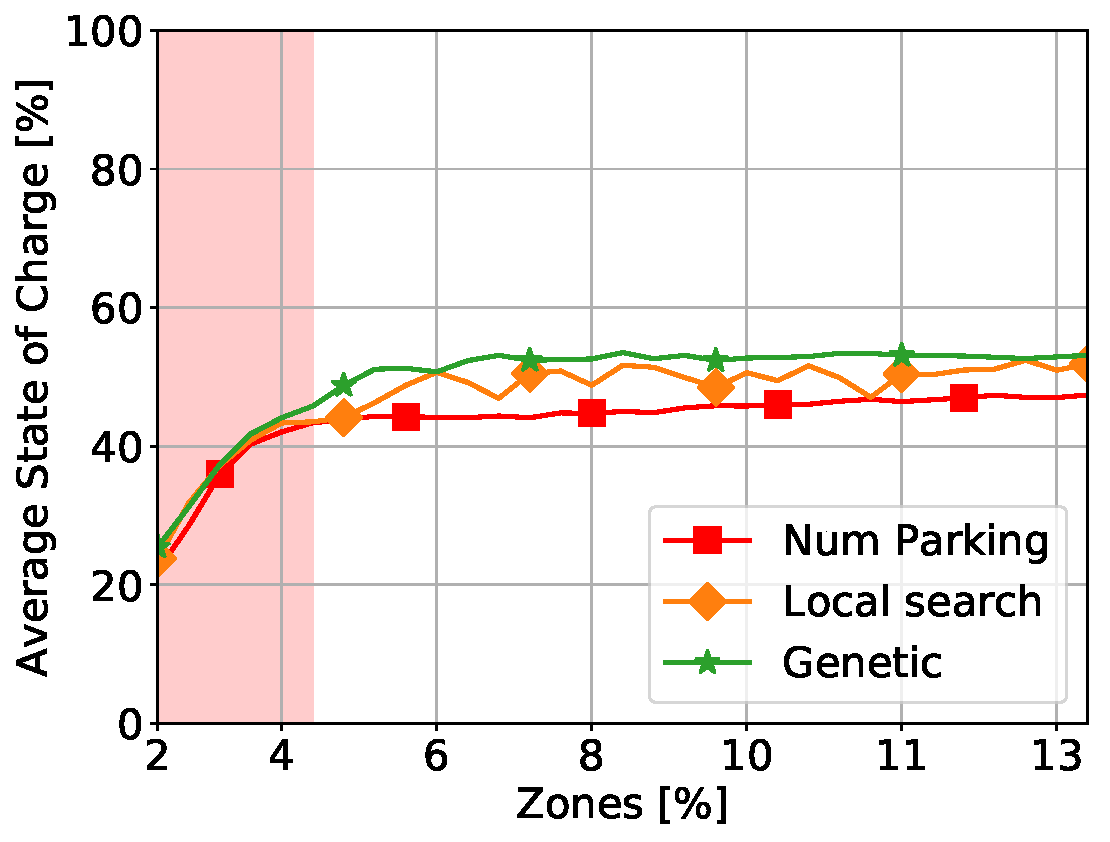
\includegraphics[width=0.45\textwidth]{figures/AvgSOC_comparison_N}
        \label{fig:asoc_Needed}
    }     
     \subfloat[][Rerouted trips percentage.]
     {
         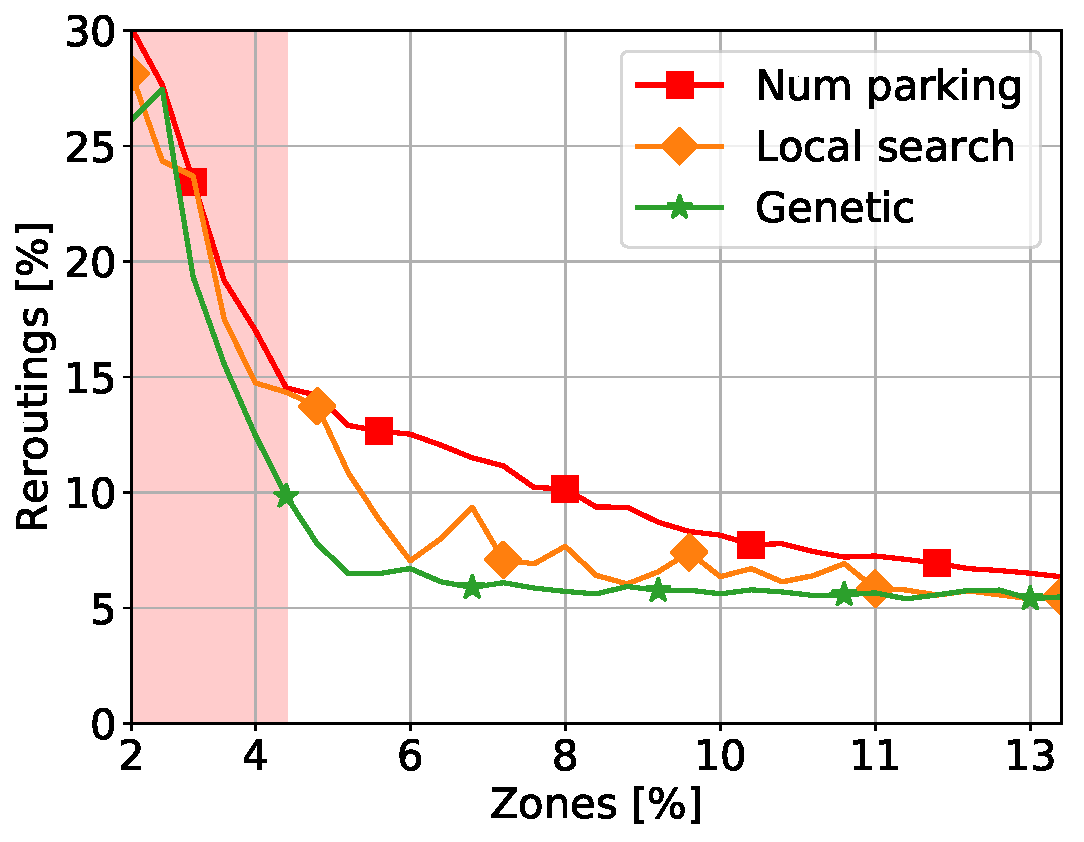
\includegraphics[width=0.45\textwidth]{figures/Needed_ReroutePerc.pdf}
         \label{fig:reroute_Needed}
     }
     \quad
     \subfloat[][Walked distance when rerouted.]
     {
         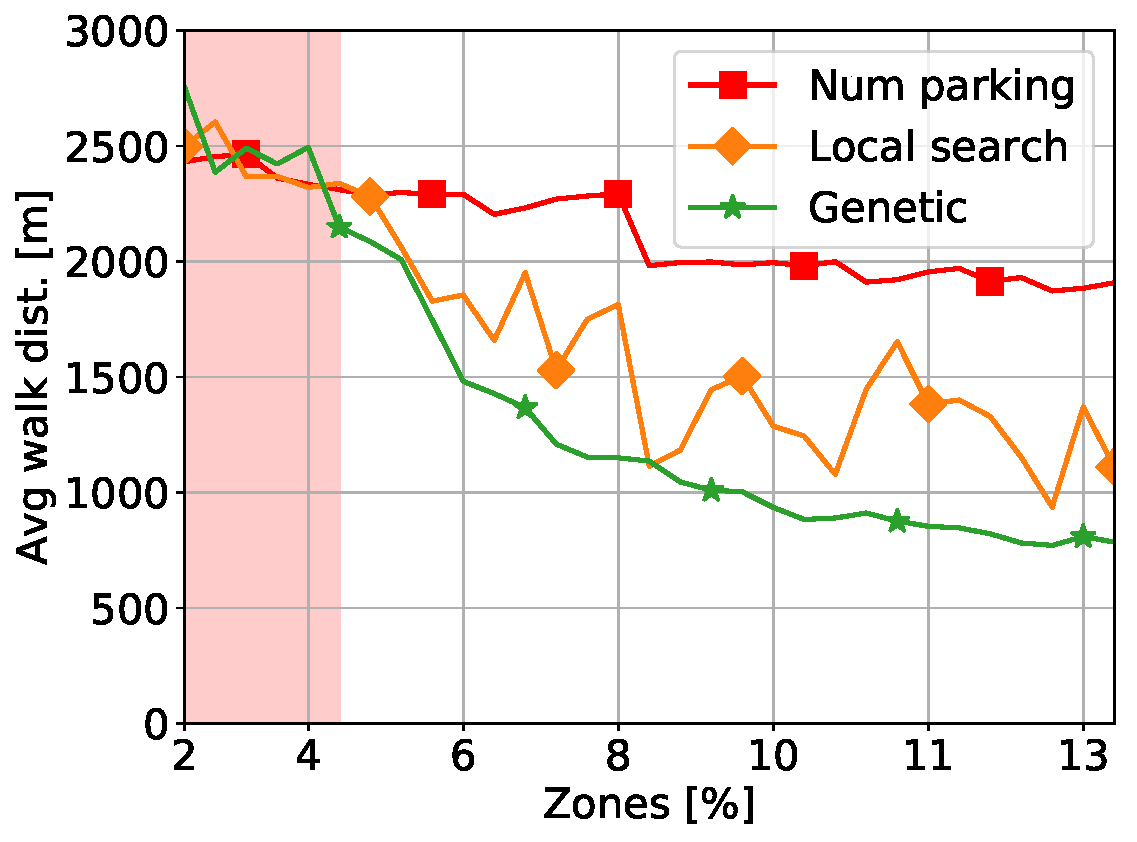
\includegraphics[width=0.47\textwidth]{figures/Needed_AvgWalkedDistance.pdf}
         \label{fig:awd_Needed}
     }
     \caption{\textit{Genetic} and \textit{local search} optimization results for metrics of interests (\textit{Needed} return policy adopted).}
     \label{fig:opt_needed}
 
\end{figure}
 
Fig~\ref{fig:opt_needed} reports the other user discomfort metrics.
The two optimisation algorithms reduce the charge events (Fig~\ref{fig:recharge_Needed}).
%The \textit{Genetic} algorithm shows the best performance with a probability the lowest probability of 6\% when 13\% of the zones are equipped with charging stations. 
%Since the car are recharged less frequently with respect to the \textit{Hybrid} policy it is interesting to evaluate the impact on the \textit{Average Stage of Charge}. Fig.~\ref{fig:asoc_Needed} reports this metric for the different placement algorithms.  As we expected, the \textit{Average Stage of Charge} is lower with respect to the \textit{Hybrid policy}. Interestingly, for both optimized solutions this value saturate almost immediately at \dg{55}\% in the feasible region. Moreover, despite in Fig.~\ref{fig:recharge_Needed} we saw that in the optimized solutions we recharge less frequent the car, 
However,  the average state of charge (Fig.~\ref{fig:asoc_Needed}) is always higher in the optimised solutions than in the \textit{Num parking} configuration. This further demonstrates that a smarter placement allows the car to get more energy for each charge.
%with an opposite trend with respect to Fig~\ref{fig:recharge_Hybrid},
%Finally, we evaluate the users discomfort metrics in terms of rerouting probability and the average distance an user has to walk when rerouted.
Fig.~\ref{fig:reroute_Needed} reports the rerouting percentage for the different algorithms. As expected, the values are larger than with the \textit{Hybrid} policy, since no opportunistic charge is performed. 
%This different is particularly evident when a few charging stations are present e.g., with 5\% of charging stations the rerouting are \dg{14}\% for the \textit{Num parking} heuristic, \dg{14}\% for the \textit{Local search}, and \dg{6}\% for the \textit{Genetic} algorithm. 
However, the genetic algorithm is able to quickly reach a small value of reroutings, hence better exploiting every charge possibility. 
%without showing further improvements while increasing the percentage of charging stations applied. 
Finally, we analyse the distance a user has to walk when rerouted (Fig.~\ref{fig:awd_Needed}). Here, with respect to the \textit{Hybrid} policy case, the \textit{local search} shows larger deviations from the \textit{Num parking}. The genetic algorithm reaches values of about 800\,m, even below the ones reached with the \textit{Hybrid} policy.

In conclusion, within this range of zones equipped with charging stations, a smart placement with the \textit{Needed} policy approaches the \textit{Hybrid} policy results.  
%Therefore, anche se gli utenti non sono tutti collaborativi, il sistema va bene lo stesso se ottimizzato.



 
 
 
 


